
%(BEGIN_QUESTION)
% Copyright 2010, Tony R. Kuphaldt, released under the Creative Commons Attribution License (v 1.0)
% This means you may do almost anything with this work of mine, so long as you give me proper credit

A type of density gauge called a {\it hydrometer} often used to measure the acid concentration in lead-acid battery electrolyte uses a weighted float with a graduated scale at the top, designed to be read at the interface between liquid and air:

$$\includegraphics[width=15.5cm]{i00282x01.eps}$$

Regarding the graduated scale at the top of the float, would the larger numbers (representing greater density) be located toward the top of the scale, or toward the bottom of the scale?  Explain your answer.

\vskip 20pt \vbox{\hrule \hbox{\strut \vrule{} {\bf Suggestions for Socratic discussion} \vrule} \hrule}

\begin{itemize}
\item{} A good problem-solving technique to apply to this is {\it limiting cases}, where you imagine extreme variations to make the problem simpler to solve.  How might you apply ``limiting cases'' to this particular problem?
\item{} Hydrometers were traditionally used in the alcohol industries to measure the strength (``proof'') of an alcohol sample.  Why do you think this method works, since a hydrometer primarily measures {\it density}?
\item{} High-accuracy hydrometers have thermometers built in so they can sense the temperature of the liquid sample.  Explain what temperature has to do with density measurement by invoking a ``thought experiment'' to see how temperature affects the reading taken by a hydrometer.
\end{itemize}

\underbar{file i00282}
%(END_QUESTION)





%(BEGIN_ANSWER)

The larger numbers (greater density) would be located at the {\it bottom} end of the scale, because liquids of greater density will cause the float to rise higher.  Liquids of low density will cause the float to sink further (with the liquid interface resting near the top of the scale).

$$\includegraphics[width=15.5cm]{i00282x02.eps}$$

This is why people float better when swimming in the Great Salt Lake of Utah than they do swimming in fresh water (or even ocean water, which is not nearly as salty).  Salt(ier) water is denser than fresh(er) water, which means a person's body need not sink as deeply to displace enough weight of water to remain buoyant.

If a person tried to swim in a vat of alcohol, where the liquid density is quite a bit less than water, they would probably drown because it would be much more difficult to achieve buoyancy.  This, however, might be a dream come true for some . . .

%(END_ANSWER)





%(BEGIN_NOTES)

\vfil \eject

\noindent
{\bf Prep Quiz:}

Which of these hydrometers is measuring the liquid of {\it least density}?

$$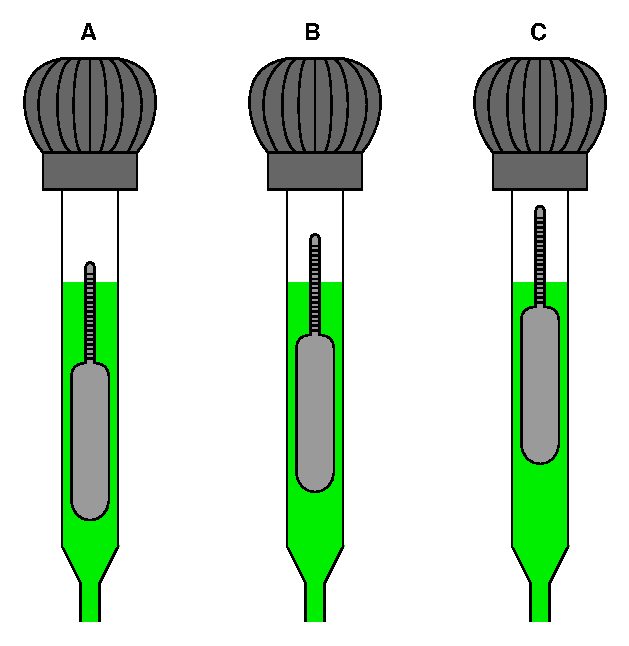
\includegraphics[width=15.5cm]{i00282x03.eps}$$

\vfil \eject

\noindent
{\bf Prep Quiz:}

Which of these hydrometers is measuring the liquid of {\it greatest density}?

$$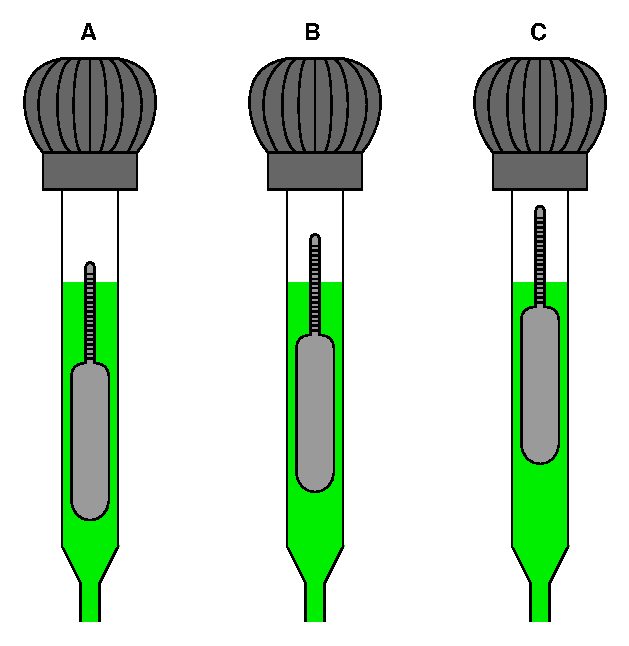
\includegraphics[width=15.5cm]{i00282x03.eps}$$


%INDEX% Measurement, density: float-type densitometer

%(END_NOTES)


